%%%%%%%%%%%%%%%%%%%%%%%%%%%%%%%%%%%%%%%%%%%%%%%%%%%%%%%%%%%%%%%%%%%%%%%%%%%%%%%
\section{Test Case 1: Pin Cell with Slowing Down Source}
\label{sec:test-case1}
%%%%%%%%%%%%%%%%%%%%%%%%%%%%%%%%%%%%%%%%%%%%%%%%%%%%%%%%%%%%%%%%%%%%%%%%%%%%%%%

%%%%%%%%%%%%%%%%%%%%%%%%%%%%%%%%%%%%%%%%%%%%%%%%%%%%%%%%%%%%%%%%%%%%%%%%%%%%%%%
\subsection{Benchmark Problem}
\label{subsec:benchmark-case1}

The first test case modeled a simple benchmark problem in which the reference flux could be computed precisely to demonstrate the existence of errors from approximately collapsing Eqn.~\ref{eqn:transport-eqn-ce} into Eqn.~\ref{eqn:transport-eqn-mg-separate} with the flux separability approximation. The first test case problem consisted of a unit cell of an infinite array of unclad fuel pins. The fuel material contained U-238 with an atom density of 0.022 $\nicefrac{\text{a}}{\text{b-cm}}$ and a purely scattering nuclide with a constant cross section of 0.176 cm\textsuperscript{-1}, an analog to oxygen in UO\textsubscript{2}. The moderator was a pure scatterer with a constant cross section of 1.23 cm\textsuperscript{-1}. The pin radius was 0.4 cm and the pitch was 1.26 cm. The source was given by the scatter source from the narrow resonance approximation:

\begin{dmath}
\label{eqn:test-source-ce}
Q(\mathbf{r},\mathbf{\Omega},E) = \frac{1}{4\pi} \frac{\Sigma_{p}(\mathbf{r})}{E} \quad .
\end{dmath}


%%%%%%%%%%%%%%%%%%%%%%%%%%%%%%%%%%%%%%%%%%%%%%%%%%%%%%%%%%%%%%%%%%%%%%%%%%%%%%%
\subsection{Simulation Tools}
\label{subsec:sim-tools-case1}

A reference continuous energy flux was computed for the this benchmark problem by solving Eqn.~\ref{eqn:transport-eqn-mg-separate} for each energy point using a method of characteristics solver with 32 azimuthal angles and a 0.01 cm ray spacing. The reference reaction rates in each region were obtained by integrating the flux multiplied by a cross section over an energy range of interest and over the volume of the fuel pin. The total cross section and source were collapsed using the reference flux according to Eqns.~\ref{eqn:sigt-mg-scalar} and~\ref{eqn:groupwise-source}, respectively. Eqn.~\ref{eqn:transport-eqn-mg-separate} was solved using the same solver with the collapsed total cross section and source. The collapsed reaction rate was obtained by volume-integrating the multi-group flux multiplied by the multi-group cross section over the fuel pin. Finally, the reaction rates obtained from the multi-group and reference calculations were compared in each energy group to identify any bias due to the flux separability approximation.

%%%%%%%%%%%%%%%%%%%%%%%%%%%%%%%%%%%%%%%%%%%%%%%%%%%%%%%%%%%%%%%%%%%%%%%%%%%%%%%
\subsection{Results and Discussion}
\label{subsec:results-case1}

This simple problem was solved for each of the resonance groups of the CASMO 70 group structure \citep{rhodes2006casmo}, which coincide with the resonances groups of the WIMS69 group structure \citep{knott2010lattice}.  Tabulated reaction rate errors are shown in \autoref{tab:case1-bias}, and the errors are presented in graphical form alongside the U-238 cross section in \autoref{fig:case1-error}.  The condensation errors range from 0.1\% in the high energy groups to just over 1\% in the lower energy groups, with the exception of Group 26.  Group 26 sits between the two lowest-lying resonances in U-238 and contains no resonances.  This suggests that these condensation errors are driven by improper accounting for self-shielding effects.

\begin{table}[h!]
  \centering
  \caption{U-238 resonance range reaction rates for collapsed cross sections on simple pin-cell.}
  \label{tab:case1-bias} 
  \begin{tabular}{c c c c c}
  \toprule
  \textbf{Group} & \textbf{\boldmath$E_{max}$ [eV]} & \textbf{Reference} & \textbf{Condensed} & \textbf{Error [\%]} \\
  \midrule
  15 & 9118.00 & 0.12018 & 0.12034 & 0.129 \\
  16 & 5530.00 & 0.11011 & 0.11030 & 0.175 \\
  17 & 3519.10 & 0.11407 & 0.11453 & 0.404 \\
  18 & 2239.45 & 0.10581 & 0.10641 & 0.567 \\
  19 & 1425.10 & 0.11572 & 0.11639 & 0.575 \\
  20 & 906.899 & 0.21110 & 0.21187 & 0.365 \\
  21 & 367.263 & 0.22169 & 0.22324 & 0.699 \\
  22 & 148.729 & 0.16551 & 0.16679 & 0.775 \\
  23 & 75.5014 & 0.10569 & 0.11216 & 0.647 \\
  24 & 48.0520 & 0.14256 & 0.14433 & 1.240 \\
  25 & 27.7000 & 0.13732 & 0.13906 & 1.270 \\
  26 & 15.9680 & 0.09348 & 0.09348 & 0.001 \\
  27 & 9.87700 & 0.23567 & 0.23883 & 1.340 \\
  \bottomrule
\end{tabular}
\end{table}

\begin{figure}
  \centering
  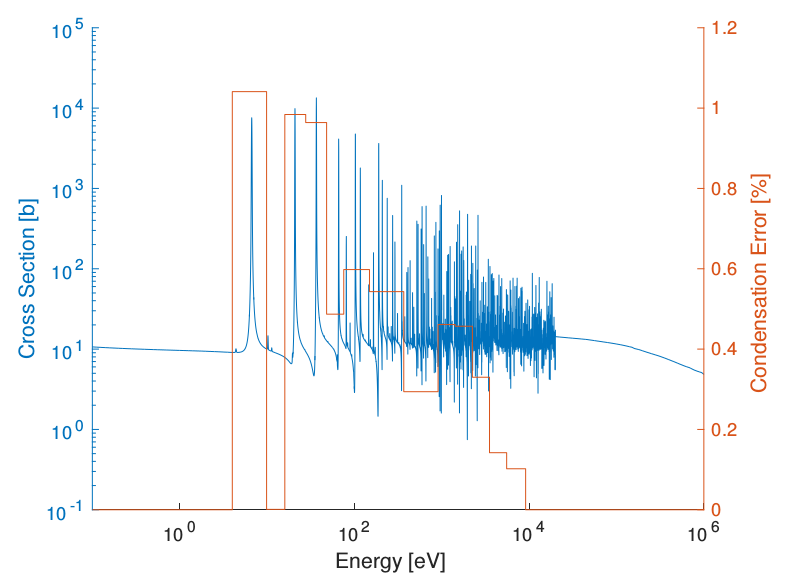
\includegraphics[width=\linewidth]{figures/case1-error}
  \caption{Condensation errors in the resonant groups of the CASMO 70 group structure, plotted alongside the U-238 cross section.}
  \label{fig:case1-error}
\end{figure}

To understand the cause of these errors, consider how neutrons reach a certain region of a fuel pin.  For a region of interest on the exterior of a fuel pin, neutrons may enter directly from the moderator or they may traverse a portion of the fuel pin first, as depicted in \autoref{fig:incoming-outgoing}.  The former are unshielded, and the spectrum is that of the asymptotic spectrum, approximately $1/E$.  The latter, however, are heavily shielded, and the spectrum will have a large depression at the resonance energy.  Thus, the resonance reaction rate and the corresponding multi-group cross section will be much larger for the first case than the second.

\begin{figure}
  \centering
  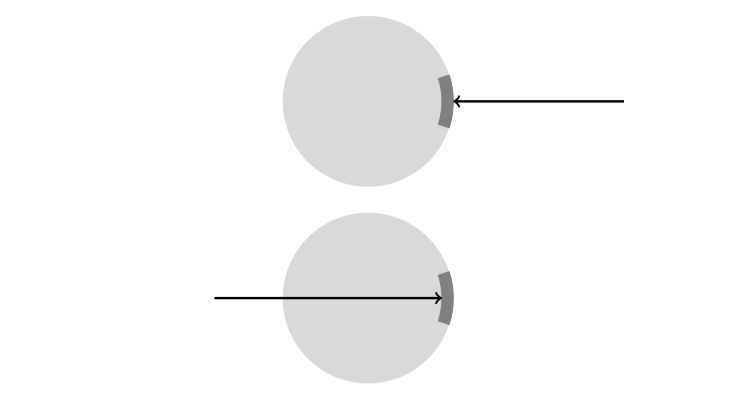
\includegraphics[width=1.15\linewidth]{figures/incoming-outgoing}
  \caption{Angular flux impinged on an FSR from the moderator (top) and after traversing the fuel (bottom).}
\label{fig:incoming-outgoing}
\end{figure}

In \autoref{fig:batman-plots}, the angular-flux-weighted cross sections as a function of incoming azimuthal angle are shown for two regions of interest in the 6.67 eV resonance group with a fixed, shallow polar angle.  The first region is on the exterior of the fuel pin and is indicated by the darkly shaded region in the upper half of the figure.  The cross section for angles in which neutrons enter from the moderator are all above 30~b, whereas the cross section for neutrons having traversed the fuel pin are as low as 5~b.  The peaks near 60\textsuperscript{o} and 120\textsuperscript{o} are due to the square array of pins; at these angles, neutrons can traverse more moderator between pins than at 90\textsuperscript{o}.  The second region is in the interior of the fuel pin and is indicated by the darkly shaded region in the lower half of the figure.  It exhibits the same characteristics of the first region, but the effects are more muted.  The maximum value of the cross section is only 15~b, and the minimum value is 5~b.  A region at the very center of the fuel pin would exhibit almost no angular dependence, as it would be shielded similarly from all directions.

\begin{figure}
\begin{subfigure}{.45\textwidth}
  \centering
  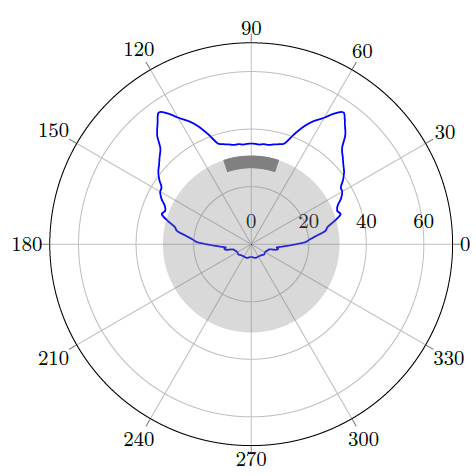
\includegraphics[width=0.8\linewidth]{figures/batman-1}
  \caption{}
  \label{fig:batman-plots-a}
\end{subfigure}
\begin{subfigure}{.45\textwidth}
  \centering
  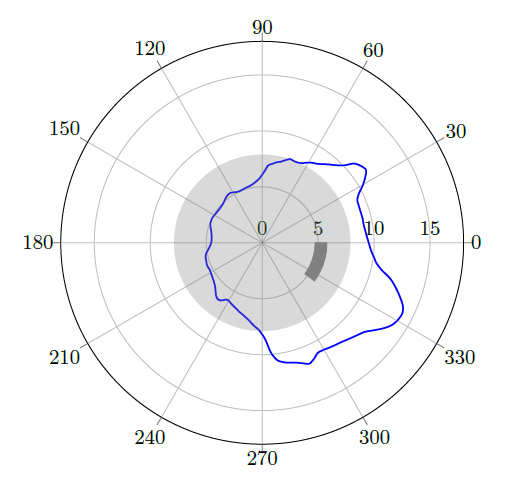
\includegraphics[width=0.8\linewidth]{figures/batman-2}
  \caption{}
  \label{fig:batman-plots-b}
\end{subfigure}
\caption{Angularly-dependent capture MGXS for the 6.67 eV resonance group as a function of azimuthal angle for two different flat source regions \citep{gibson2016thesis}. The radial axis is given in units of barns and the azimuthal axis in units of degrees.}
\label{fig:batman-plots}
\end{figure}
